\chapter{Komparator LM311}

\section{Budowanie układu}

\begin{itemize}
    \item Należało zbadać komparator \textbf{LM311} korzystając z płytki UA-1.
        \begin{figure}[H]
            \centering
            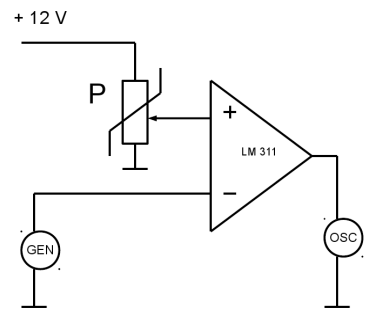
\includegraphics[width=0.5\textwidth]{img/schemes/1.png}
            \caption{Schemat budowanego układu}
            \label{komparator:schemat}
        \end{figure}
    \item Korzystając ze schematu wyżej (\ref{komparator:schemat}) zmontowano układ. Skorzystano z opornika znajdującego się na płytce UA-1, który za pomocą pokrętła został dynamicznie zmieniany.
    \item Skorzystano z trójnika aby do oscyloskopu przesyłać sygnał z generatora (GEN) oraz wyjściowy z komparatora (OSC).
        \begin{figure}[H]
            \centering
            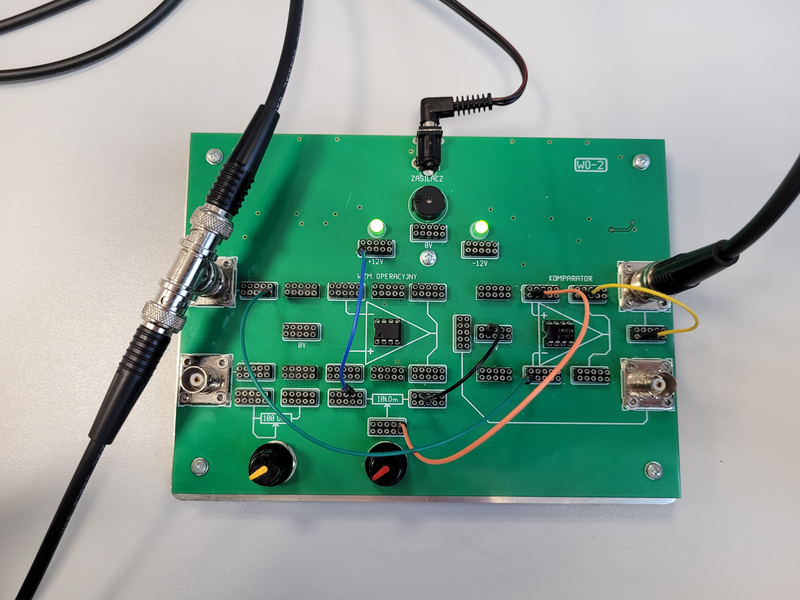
\includegraphics[width=0.8\textwidth]{img/1/20220608_085306_scaled.png}
            \caption{Zbudowany układ z komparatorem LM311}
            \label{komparator:zbudowany}
        \end{figure}
\end{itemize}

\section{Testowanie układu}

\begin{itemize}
    \item Zbudowany układ generował sygnał prostokątny na wyjściu.
        \begin{figure}[H]
            \centering
            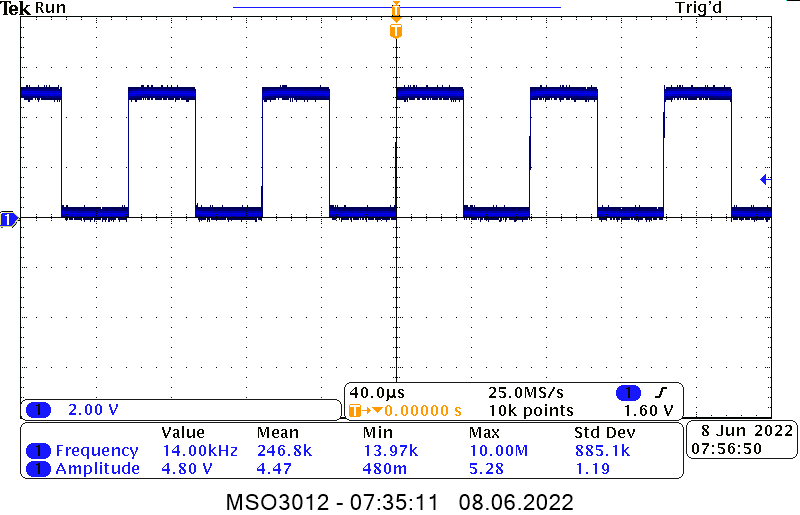
\includegraphics[width=0.8\textwidth]{img/1/1_dzialajacy_cropped.png}
            \caption{}
            \label{fig:my_label}
        \end{figure}
    \item Dodatkowo przetestowano układ dla różnych kształtów fali sygnału wchodzącego do układu (sygnał wejściowy o parametrach: 5V 14kHz) przy wartości P = 9.82k$\Omega$.
        \begin{figure}[H]
            \centering
            \begin{subfigure}[H]{0.48\textwidth}
                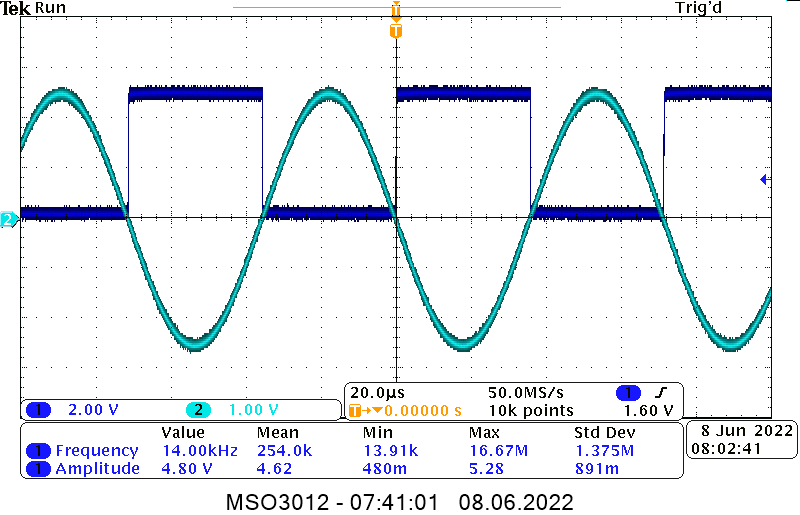
\includegraphics[width=\textwidth]{img/1/1_wejscie_wyjscie_cropped.png}
            \end{subfigure}
            \begin{subfigure}[H]{0.48\textwidth}
                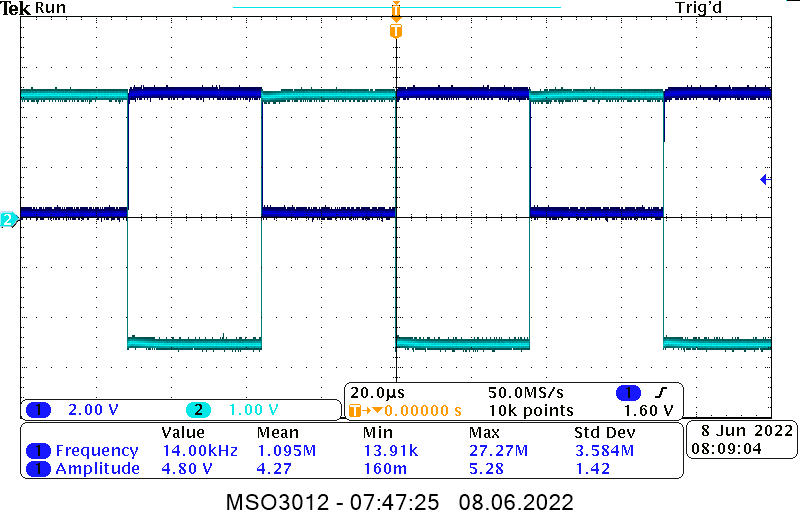
\includegraphics[width=\textwidth]{img/1/1_kwadratowa_cropped.png}
            \end{subfigure}
            \begin{subfigure}[H]{0.48\textwidth}
                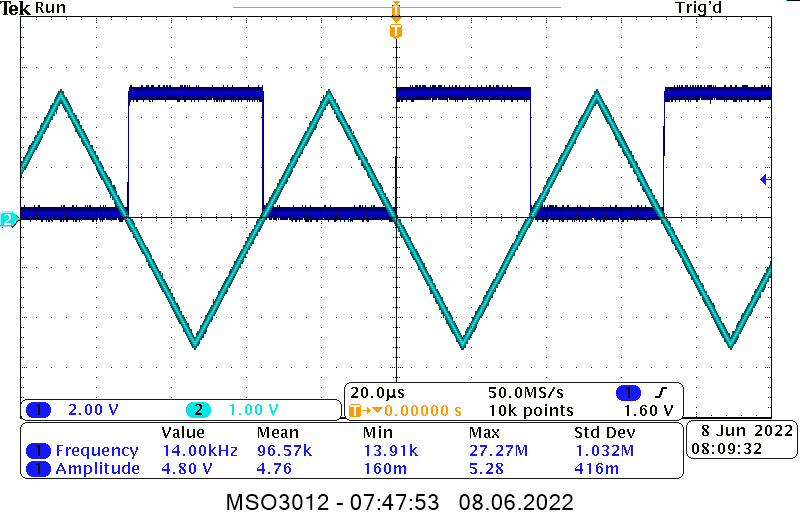
\includegraphics[width=\textwidth]{img/1/1_trojkat_cropped.png}
            \end{subfigure}
        \end{figure}
        Kształt fali wejściowej nie wpływa na wyjście komparatora.
    \item Następnie zbadano zachowanie układu na zwiększoną częstotliwość sygnału wejściowego.
        \begin{figure}[H]
            \centering
            \begin{subfigure}[H]{0.48\textwidth}
                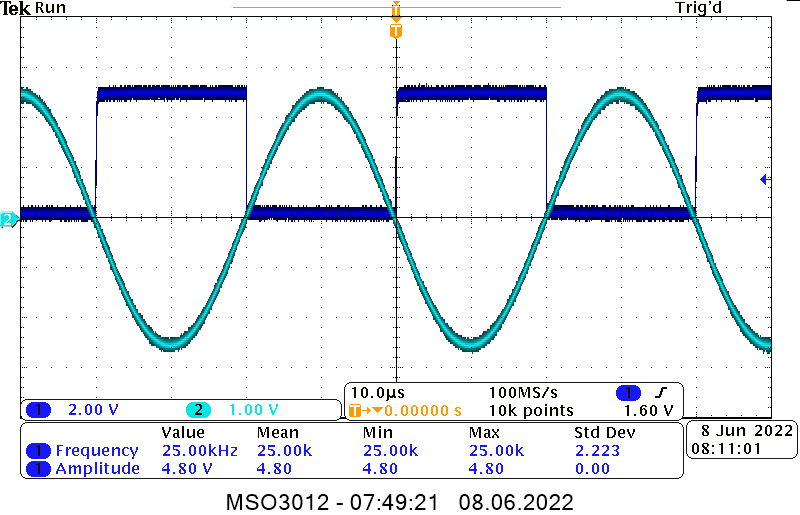
\includegraphics[width=\textwidth]{img/1/1_25khz_cropped.png}
                \caption*{f = 25kHz}
            \end{subfigure}
            \begin{subfigure}[H]{0.48\textwidth}
                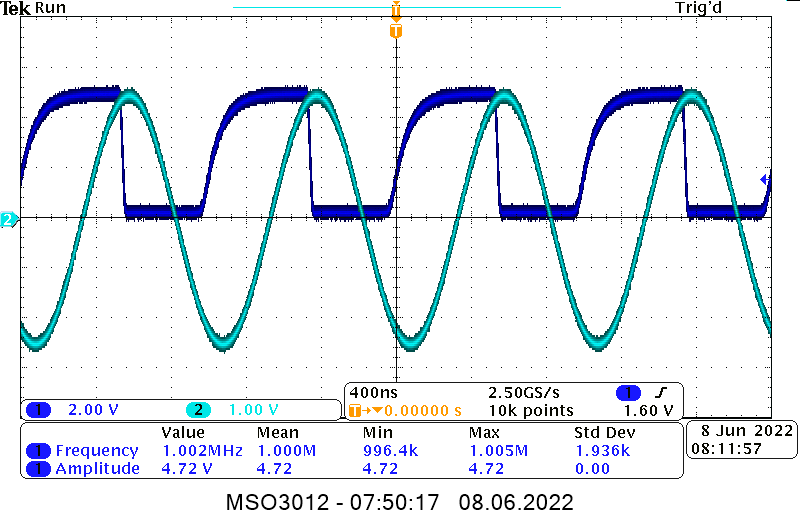
\includegraphics[width=\textwidth]{img/1/1_1mhz_cropped.png}
                \caption*{f = 1MHz}
            \end{subfigure}
        \end{figure}
        Dla wysokich czestotliwości (\textbf{>1Mhz}) komparator nie zdążył w pełni przetworzyć sygnału wejściowych.
    \item Ostatnią częścią było sprawdzenie granicznej wartości \textbf{P}, dla której sygnał wyjściowy pozostawał niezmienny.
        \begin{figure}[H]
            \centering
            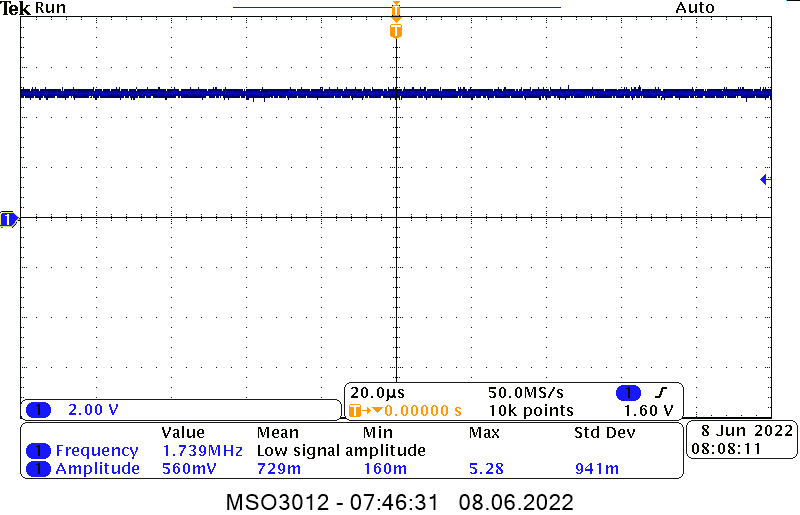
\includegraphics[width=0.6\textwidth]{img/1/1_prosta_linia_cropped.png}
        \end{figure}
        Wartość P została zmierzona \textbf{multimetrem} i wyniosła \textbf{P = 7.78k$\boldsymbol{\Omega}$}
    \item Komparator działał \textbf{poprawnie}.
\end{itemize}